
\chapter{GPGPU}

With high demand for real-time image processing, computer vision applications and a need for fast calculations in the scientific world, general-purpose computing on GPU (Graphics Processor Units), also known as the GPGPU, has become a popular programming model to accelerate programs traditionally coded on the CPU (Central Processing Unit).

Until the last decade or so, when technologies for GPGPU became available, the GPU was used mostly to render data given to it by the CPU. This has changed in a way, that the GPU, with its massive parallel capabilities, isn't used only for displaying, but also for computation. The approach to this is to transfer data bidirectionally between the CPU and the GPU, which on one hand brings the overhead of copying the data, but on the other enables to do the calculations many times faster due to the architecture of the GPU. As shown on \ref{fig:cpu-gpu} many more transistors are dedicated to data processing instead of cache or control, which leads to a higher memory bandwidth.

\begin{center}
\begin{figure}[h]
	\centering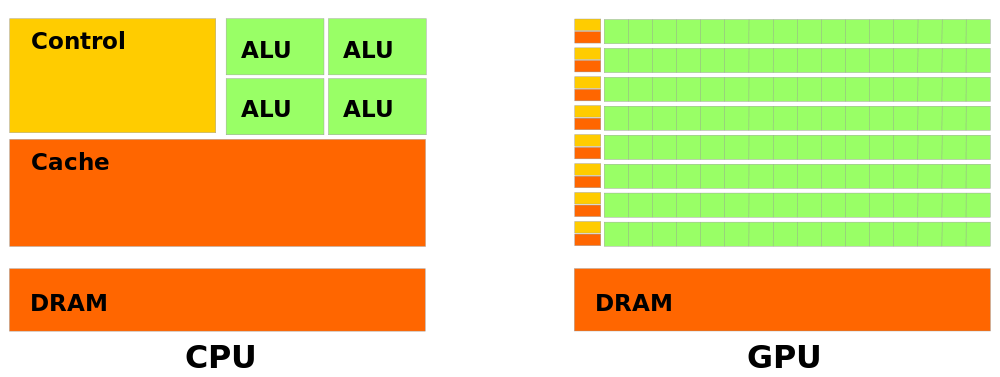
\includegraphics[height=5cm]{fig/cpu-gpu.png}
	\caption{CPU and GPU architecture comparison (\cite{cuda-toolkit-docs})}
	\label{fig:cpu-gpu}
\end{figure}
\end{center}

GPUs are also designed with floating-point calculations in mind, which can be taken advantage of, in applications such as object detection, where most of the math is done using single-precision floating-point arithmetic.

\begin{center}
\begin{figure}[h]
	\centering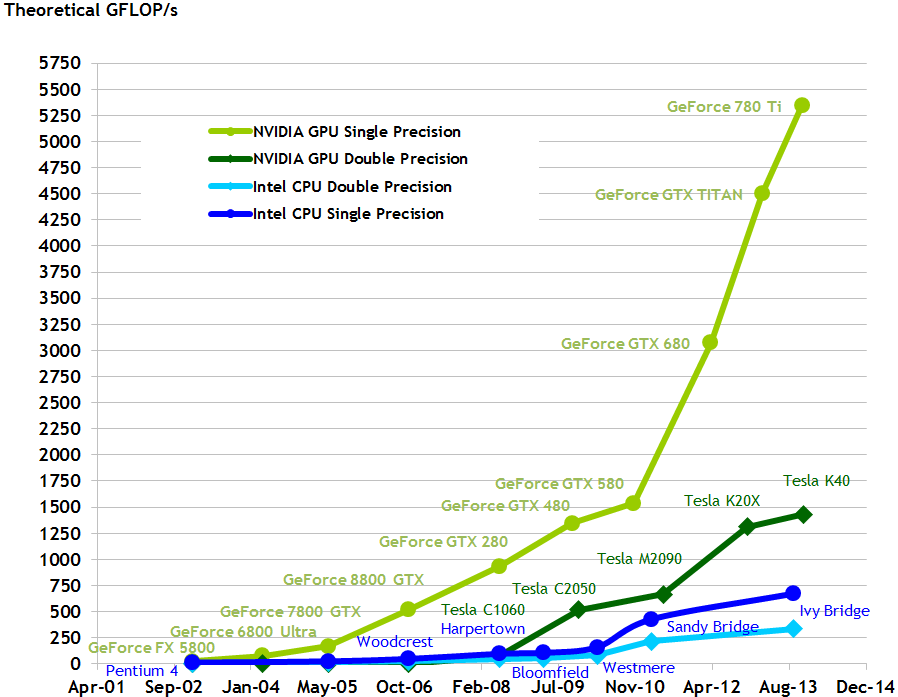
\includegraphics[height=10cm]{fig/floating-point-operations-per-second.png}
	\caption{Floating-Point operations per second for the CPU and GPU (\cite{cuda-toolkit-docs})}
\end{figure}
\end{center}

\section{Parallel computing platforms}

In November 2006 the first parallel computing platform - CUDA (Compute Unified Device Architecture) was introduced by NVIDIA. Since then the world of GPUs and computer graphics have changed significantly. The GPU stopped to be viewed only as a tool for displaying, but became another processing unit. By introducing CUDA to programmers, suddenly its programming model and memory model became available for use. 

The most widely used GPGPU platforms are the following.

\begin{itemize}
	\item CUDA - NVIDIA
	\item OpenCL - Khronos Group
	\item C++ AMP - Microsoft	
	\item Compute shaders - OpenGL
	\item DirectCompute - Microsoft
\end{itemize}

All of the technologies above allow access to the GPU computing capabilities. The first two - CUDA and OpenCL work on a kernel basis. As a programmer, you have access to low-level GPU capabilities and have to manage all the resources yourself. The standard approach is the following:

\begin{enumerate}
	\item Allocate memory on the GPU
	\item Copy data from the CPU to the allocated memory on the GPU
	\item Run a GPU based kernel (written in CUDA or OpenCL)
	\item Copy processed data back from the GPU to the CPU
\end{enumerate}

C++ AMP is a more higher-level oriented library. Introduced by Microsoft as a new C++ feature for Visual Studio 2012 with STL-like syntax, it is designed to accelerate code using massive parallelism. Currently it is supported by most GPUs, which have a DirectX 11 driver.

The last two - Compute shaders and DirectCompute also work in a more high-level fashion, but quite differently from C++ AMP. They are not a part of the rendering pipeline, but can be set to be executed together with other OpenGL or DirectX shaders.

\subsection{Evolution of the graphics pipeline}

This change towards a more general-purpose use of GPUs can be also viewed in the current OpenGL pipeline, with which most graphics programmers are familiar. In OpenGL 2.0 (2004) shader programs were introduced enabling to partially program the pipeline itself. With OpenGL 3.* (2008-2010) the shader language had improved significantly and geometry shaders were introduced. Later on in 2010 another programmable stage was introduced with OpenGL 4.0 - the tesselation shader, but still these were set stages with a predefined purpose. The most significant year for the GPGPU was 2012 with OpenGL 4.3 and the Compute Shaders. 

Compute shaders are very specific. They don't have a set number of inputs, outputs or a place in the pipeline. It is up to the programmer to specify these and also to specify a space on which they operate, like per-pixel or per-vertex basis, by fetching the data itself. This means that even the graphics pipeline, traditionally used for visualization, changed in a way, that it can be programmed without the use of traditional shaders, with compute shaders only and a more general-purpose use in mind.

\section{NVIDIA CUDA}

NVIDIA CUDA is a programming model enabling direct access to the instruction set and memory of NVIDIA GPUs. The other main competitor to CUDA, on the market, is OpenCL. Both of these models are designed with direct access to the GPU's capabilities in mind compared to other parallel platforms. OpenCL has the advantage of not being platform specific. It is supported by both major GPU vendors AMD and NVIDIA. CUDA is only usable on NVIDIA cards, but generally offers more options to the programmer and a better debugging environment.

\subsection{Programming model}

CUDA uses a language called CUDA C, which is an extension to C and uses NVCC compiler to generate code for the GPU. It also allows to write C-like functions called kernels. A kernel is defined by the \verb|__global__| declaration specifier and is executed using a given configuration wrapped in \verb|<<< ... >>>|. The configuration is specifies a grid and takes as parameters the number of blocks and the number of threads per block. The same kernel code is run by the whole grid. Code run by the kernel on the GPU is called the device code, whereas the code run outside of the kernel by the CPU is called the host code.

\subsubsection{Thread hierarchy}\label{subsubsec:thread-hierarchy}

\paragraph{Threads} are a basic computational unit uniquely identified by 3-dimensional indexes \verb|threadIdx| (an index within a block) and \verb|blockIdx| (an index of a block).

\paragraph{Blocks} are groups of threads, where every block resides on a single processor core, therefore a kernel can be run with the maximum of 1024 threads. Each block is uniquely identified by a 3-dimensional index \verb|blockIdx|. Threads within a block can be synchronized by a \verb|__syncthreads| call, but blocks themselves can't be synchronized, and so a new kernel must be run to do so.

The code is executed in a SIMT (Single Instruction, Multiple Thread) fashion, which is very similar to the commonly known SIMD (Single Instruction, Multiple Data) architecture. In reality the code is executed in groups of 32 threads, referred to as warps and a single Kepler or Maxwell multiprocessor supports up to 64 active warps. The important thing to mention about warps is, that when a single thread within a warp is active, the whole warp stays active and so performance-wise it is important to optimize the code to occupy warps as much as possible.

\begin{center}
\begin{figure}[h]
	\centering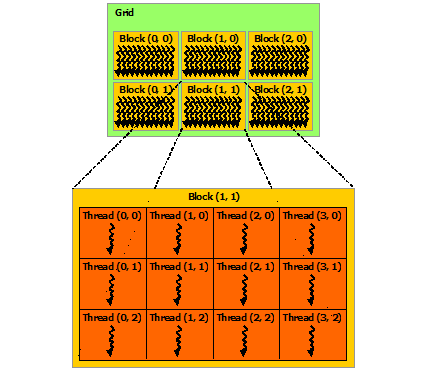
\includegraphics[height=5.5cm]{fig/grid-of-thread-blocks.png}
	\caption{A grid of blocks and threads run by a kernel (\cite{cuda-toolkit-docs})}
\end{figure}
\end{center}

Kernel configuration parameters can be passed as integers or \verb|dim3| structures. \verb|dim3| specifies the number of threads or blocks in every dimension, therefore a \verb|dim3 threadsPerBlock(4,4,1)| would run a kernel with 16 threads per block, where \verb|threadIdx.x| would range between 0 and 3 and the same for \verb|threadIdx.y|.

Example \ref{code:cuda-example} shows how to add 2 arrays in parallel using N threads and 1 block.

\begin{figure}[h]
\begin{verbatim}
// Kernel definition
__global__ void VecAdd(float* A, float* B, float* C)
{
    int i = threadIdx.x;
    C[i] = A[i] + B[i];
}

int main()
{
    ...
    // Kernel invocation with N threads
    VecAdd<<<1, N>>>(A, B, C);
    ...
}
\end{verbatim}

\caption{Example of vector addition in CUDA (\cite{cuda-toolkit-docs})}
\label{code:cuda-example}
\end{figure}

\FloatBarrier

\subsubsection{Scheduling}\label{subsubsec:scheduling}

After a kernel is launched, the grid is organized in blocks, grids and threads, which are described in \ref{subsubsec:thread-hierarchy}. Depending on the architecture, blocks can have only up to certain number of warps and threads (\ref{tab:capability-3050}).

\begin{table}[htbp]
\begin{center}
\begin{tabularx}{0.75\textwidth}{| X | X | X |}
\hline
Compute Capability & 3.0 & 5.0 \\
\hline
Max. number of blocks per SM & 16 & 32 \\
\hline
Max. number of warps per SM & 64 & 64 \\
\hline
Max. number of threads per SM & 2048 & 2048\\
\hline
Max. number of threads per block & 1024 & 1024\\
\hline
Local memory per thread & 512 KB & 512 KB \\
\hline
Max. shared memory per SM & 48 KB & 64 KB\\
\hline
\end{tabularx}
\end{center}
\caption{Limits of devices for Compute Capability 3.0 (Kepler) and 5.0 (Maxwell). SM stands for Streaming Multiprocessor.}
\label{tab:capability-3050}
\end{table}

Blocks are assigned between multiprocessors, where for modern GPU's, their count ranges between a single multiprocessor for average GPU's and 16 for the high-end. Threads within a block are then divided into warps. Warp execution is controller by a warp scheduler using a prioritized scheduling policy.

All threads within a warp execute the same instruction at the same time. In case the instruction is not active for the given thread, an active mask is used and as soon as all the threads within the warp finish or are stalled by synchronization, a new warp is assigned.

\begin{figure}[h]
	\begin{center}
	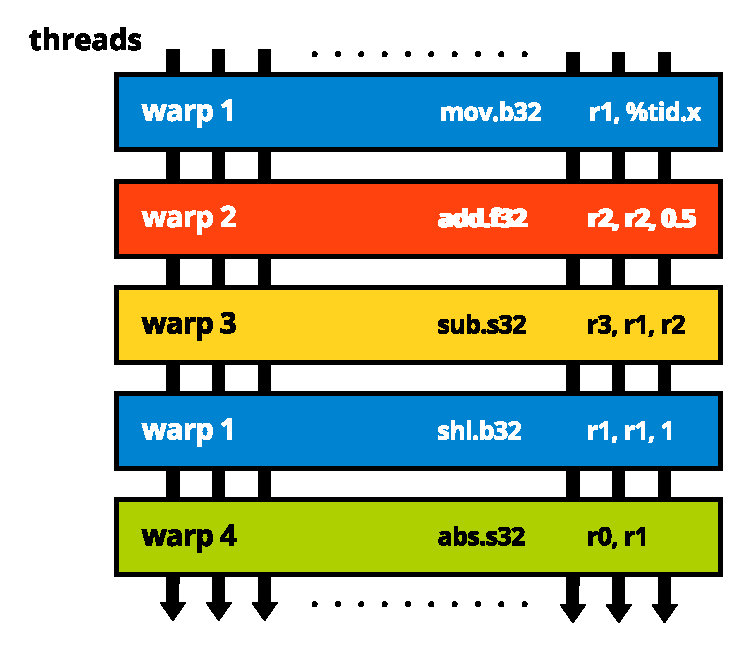
\includegraphics[width=0.4\textwidth]{fig/scheduling.eps}
	\caption{As soon as an instruction has its operands ready, it is scheduled by the warp scheduler for execution.}
	\label{fig:scheduling}
	\end{center}
\end{figure}

\subsection{Memory model}\label{subsec:memory}

Another important aspect of CUDA are the types of memories, which can be used. They range from locally accessible registers with extremely fast access to globally accessible global memory, which takes hundreds of cycles to read or write to or from. They are summarized by the following table:

\begin{table}
\centering
\begin{tabular}{| l | l | l | l | l |}
\hline
Memory & Keyword & Scope & Access & Lifetime \\
\hline
Registers & - & Thread & Read/Write & Kernel \\
\hline
Local memory & - & Thread & Read/Write & Kernel \\
\hline
Shared memory & \verb|__shared__| & Block & Read/Write &  Kernel \\
\hline
Global memory & \verb|__device__| & Grid & Read/Write & Application \\
\hline
Texture memory & - & Grid & Read-only & Application \\
\hline
Constant memory & \verb|__constant__| & Grid & Read-only & Application \\
\hline
\end{tabular}
\caption{Memory types}
\end{table}

\paragraph{Global memory} is accessible by all threads in a grid and allows both reading and writing. It is also the slowest memory type. Its access is the bottleneck for most applications with access latency ranging from 400 to 800 cycles. There are several strategies for it to be fast like coalescing access with 32-, 64-, 128-byte transactions, described in \ref{subsubsec:coalescing}.

\paragraph{Texture memory} can be regarded similarly to global memory. Cache is optimized for 2D spatial access pattern and address modes or interpolation can be used at no additional cost.

\paragraph{Constant memory} is the third memory type, which can be accessed by all threads and is typically used to store constants or kernel arguments. It doesn't bring any speed-up compared to global or texture memory, but it is optimized for broadcast, which means that it is optimal to use it, when the same data is accessed by all the blocks.

\paragraph{Shared memory} can be accessed by all threads within a block. It is much faster than the other types, but is commonly subjected to bank conflicts. It is mainly used for acceleration.

\paragraph{Unified memory} is a memory type introduced in CUDA 6.0. It enables to use the same memory addresses both in host and device code, which simplifies writing code. On the other as of spring 2014, there doesn't seem to be any hardware support \cite{unified-memory} and performance-wise the unified memory performs very similar to global memory.

\paragraph{Local memory} is a part of global memory, where everything which doesn't fit into registers is stored. For devices with Compute Capability 2.x there are 32768 32-bit registers.

\begin{center}
\begin{figure}[h]
	\centering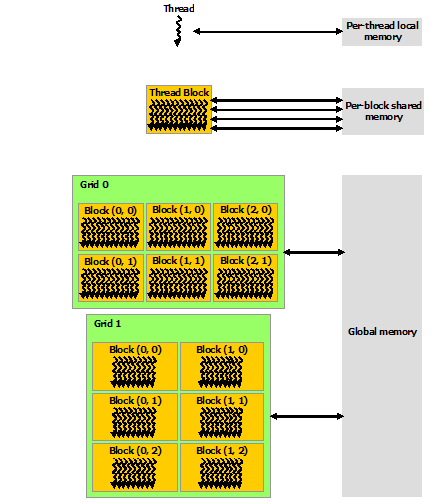
\includegraphics[height=12cm]{fig/memory-hierarchy.png}
	\caption{Memory hierarchy (\cite{cuda-toolkit-docs})}
\end{figure}
\end{center}

\subsection{Optimization methods}\label{subsec:optimization}

\subsubsection{Global memory coalescing}\label{subsubsec:coalescing}

Using global memory is generally slow, but it is unavoidable to use, because it is the only type of GPU memory, which can be copied to from the CPU. On the other hand, since Compute Capability 1.1, global memory loads and stores can be optimized by coalescing, thus making it much faster.

\begin{center}
\begin{figure}[h]
	\centering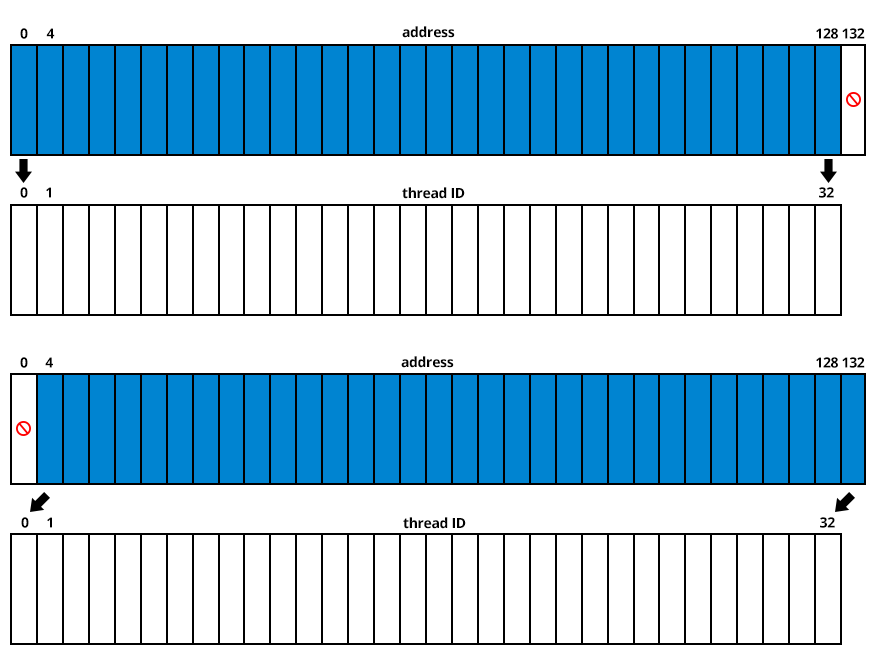
\includegraphics[width=0.6\textwidth]{fig/coalescing.png}
	\caption{Coalescing access to global memory. Top part shows coalesced access, whereas bottom part shows strided uncoalesced access.}\label{fig:coalescing}
\end{figure}
\end{center}

GPU can access memory in 32-, 64- or 128-byte transactions. Therefore, in case the memory access is aligned, multiple banks can be read or written to in a single transaction. On the other hand when it is not, more transactions have to be initialized, making the memory bandwidth much lower. Examples of coalesced (top) \ref{code:coalesced} and uncoalesced (bottom) \ref{code:uncoalesced} access with stride of 4 bytes are shown in \ref{fig:coalescing}.

\begin{figure}[h]
\begin{verbatim}
tmp = globalmem[blockIdx.x * blockDim.x + threadIdx.x];
\end{verbatim}
\caption{Example of coalesced global memory load.}\label{code:coalesced}
\end{figure}

\begin{figure}[h]
\begin{verbatim}
tmp = globalmem[blockIdx.x * blockDim.x + threadIdx.x + stride];
\end{verbatim}
\caption{Example of uncoalesced global memory load with a stride.}\label{code:uncoalesced}
\end{figure}

It is a common optimization technique, to use shared memory in cases, where strided access is needed. Data is copied between global memory and shared memory in a coalesced fashion, but then strided access is used on shared memory without a penalty.

\subsubsection{Thread synchronization and stalling}

Threads cannot be synchronized across the whole grid, but only across a block. Therefore, if a result of a certain computation is needed by all the threads, a whole new kernel has to be launched. Synchronization across a block is done by the \verb|__syncthreads| call. When a thread reaches this call, it waits idly until all the threads within the block also reach the call.

In certain scenarios, it might take a lot longer for a certain thread to process its code, then for another. An example is the prefix-sum, as described later on in \ref{sec:prefixsum}, where the number of iterations of a for-cycle depends on the thread ID. The problem is, that after the for-cycle finishes, threads must be synchronized. Most of the threads in this case are stalled and cannot be freed until all of them finish to run another warp.

When writing a kernel, it is important to keep this in mind and try to minimize the use of \verb|__syncthreads| calls, where this would lead to stalling most of the threads.

\chapter{Object detection}

\section{Introduction}

Object detection is a computer technology with the capability of localizing an object in input image data. The type of object depends on which data the detector was trained for. Typical applications are human faces, pedestrians, cars, traffic signs and others.

Detector used by the implementation is a frontal-face human detector, which tries to identify a human face within an image. The implementation is therefore optimized for human faces, which means, that the software can be used with other detectors, but it might effect its performance due to specific optimizations. Combined with the capabilities of a GPU, the aim is to produce an object detector capable of real-time object detection on videos or processing large amounts of images.

\section{Features}

There are several methods how to access the topic of object detection. In the following sections we will discuss feature-based object detection.

Let's take a frontal human face as an example. Despite the differences such as lighting, color of eyes or skin or the length of hair, we as humans, can identify we are looking at a human face based on similarities. For example a pair of eyes, a nose, a pair of ears and so on. These similarities can be called features, but to a computer, they are still too abstract and cannot be enumerated, and so a lot of different feature methods were devised.

\subsection{Local Binary Pattern}

One of the feature methods to describe an image are local binary patterns (LBP). They are based on encoding local intensities of an image with 8-bit codes. In their elementary form, they take a 3x3 area as an input and compare intensity values of all the pixels with the central one.

\[
 compare(p_{middle},p_{i}) =
  \begin{cases}
   1 & \text{if } p_{i} \geq p_{middle} \\
   0 & \text{else}
  \end{cases}
\]

LBP value is then evaluated as follows:

\begin{equation}
lbp(p_{middle})=\sum_{i=0}^{7} 2^{i}
compare(p_{middle},p_{i})
\end{equation}


\begin{center}
\begin{figure}[h]
	\centering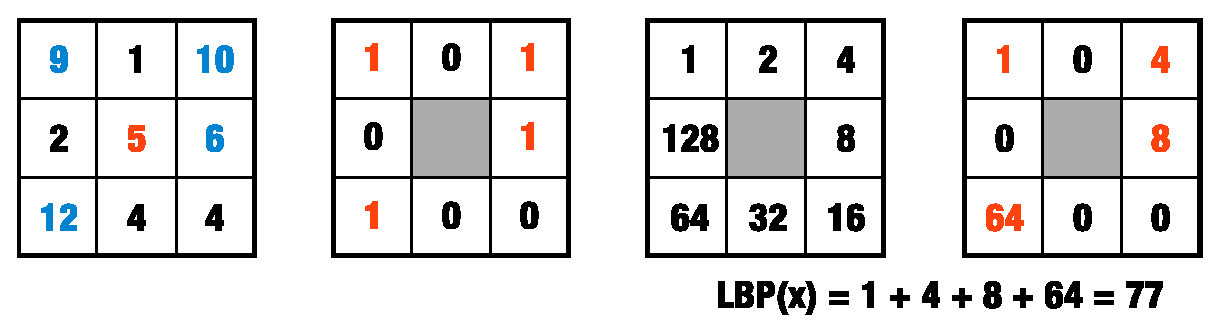
\includegraphics[width=12cm]{fig/lbp.eps}
	\caption{LBP feature}
\end{figure}
\end{center}

LBPs can be extended to be used not only for single pixels and thus 3x3 areas, but also for larger areas. When comparing larger areas, the sum of the areas is compared instead of single pixel values. For example a 2x2 LBP would sum up areas of 4 pixels and compare them with the sum in the middle.

LBP features are invariant to lighting changes, because even though the image is lighter or darker, the intensity differences stay the same. On the other hand they are not invariant to geometrical transformations such as scale or rotation.

As mentioned later on in \ref{sec:memory-organization}, the areas don't necessarily have to be summed up, but can be interpolated instead, because the LBP code generated after comparing average values and summed up values is the same.

\section{Waldboost}
\label{sec:waldboost}

Each LBP feature represents a single weak classifier, which decides whether the given sample corresponds to the sought object or not. On the other hand only one feature cannot describe the whole face, so a meta-algorithm to process a series of such weak classifiers is needed, combining them in a single strong classifier.

One such algorithm is WaldBoost, which combines AdaBoost and Wald's Sequential Propability Ratio Test (SPRT). SPRT is a strategy to determine what class a sample belongs to, based on a series of measurements.

\[
 SPRT =
  \begin{cases}
   +1 & \text{if } R_{m} \leq B \\
   -1 & \text{if } R_{m} \geq A \\
   \# & \text{else take another measurement} 
  \end{cases}
\]

$R_{m}$ is the likelihood ratio and A, B are constants to compute the wanted false negatives $\alpha$ and false positives $\beta$ ratios as follows:

\begin{equation}
R_{m}=\frac{p(x_{1}, ..., x_{m}|y=-1)}{p(x_{1}, ..., x_{m}|y=+1)}
\end{equation}

\begin{equation}
A=\frac{1-\beta}{\alpha}, B=\frac{\beta}{1-\alpha}
\end{equation}

As mentioned in \cite{sochman-matas-waldboost} with face detection in mind, the positive rate $\beta$ can be set to 0 and the required false negative rate $\alpha$ to a small constant. As such the equations can be simplified to

\begin{equation}
A=\frac{1-0}{\alpha}=\frac{1}{\alpha}, B=\frac{0}{1-\alpha}=0
\end{equation}

and the whole strategy to

\[
 SPRT =
  \begin{cases}
   +1 & \text{if } R_{m} \leq 0 \\
   -1 & \text{if } R_{m} \geq \frac{1}{\alpha} \\
   \# & \text{else take another measurement} 
  \end{cases}
\]

$R_{m}$ is always positive and therefore the algorithm will only classify the sample as a face when it finishes its training cycle or discard it as a background when the ratio gets greater than the given constant A.

\section{Uses cases of object detection}

\subsection{Face tracking and recognition}\label{subsec:face-tracking}

One of the initial releases of the detector was already used as a part of a project\footnote{\url{https://github.com/mmaci/vutbr-fit-pov-face-tracking}} for face tracking and recognition on a video, which might be a typical use case for security cameras.

In order to track a face, the face has to be recognized in the previous frames, so faces have to be detected for every frame. The detector processes the frame and outputs detections. The detections are then processed as follows:

\begin{enumerate}
	\item \textbf{Choose the best response detection.} There are usually more detections for every face, depending on the number of sub-sampled images. Out of the overlapping detections, the detection with the best response is chosen.
	\item \textbf{Coversion to HSV.} The detection (a square-sized area) is converted to HSV (Hue, Saturation, Value color model) and a histogram is calculated. For a human face, the V component can be dropped, which provides luminance invariability.
	\item \textbf{Histogram comparison.} The histogram of H and S values is compared with the histogram of all the previously found faces. The distance from the detection is also taken into consideration, because we presume the face doesn't change positions too much.
\end{enumerate}

To calculate the difference between two ROI historgram different methods can be used. In this case Bhattacharyya distance \ref{eq:bhatta}.

\begin{figure}
\begin{equation}
d(H_{1},H_{2})=\sqrt{1-\frac{1}{\sqrt{\overline{H_{1}}\overline{H_{2}}N^2}}\sum\limits_{I}\sqrt{H_{1}(I) \cdot H_{2}(I)}}
\end{equation}
\caption{Bhattacharyya distance}
\label{eq:bhatta}
\end{figure}

In order to track or recognize a face in real-time, both the detection and the recognition have to be processed faster, than the framerate.

\chapter{Analysis}

In this chapter, research done on the topic of WaldBoost object detection, in the previous years, is summarized. Also tools to choose from for the implementation and the idea how to implement the detector, are discussed. It does now however cover implementations specifics. These are discussed later on in \ref{ch:implementation}.

The idea of implementing a WaldBoost object detector with the use of LBP features on a parallel platform is not a new one and mainly for face detection, it is well researched. On the other hand, since it was first proposed, both OpenCL and CUDA have undergone many changes and as such optimizations and different approaches to the implementation can be discussed. The main focus of this thesis is to produce an implementation, which is optimized for different GPU's and to research how different uses of GPU memory and optimization techniques affect the detector.

The implementation of a WaldBoost detector on a CPU, where every pixel is processed sequentially isn't complicated. The general idea, as explained in \ref{sec:waldboost}, is that a sample, in our case a pixel, is processed by a series of weak classifiers, in the implementation called stages. These stages accumulate a response, always adding or subtracting a value based on how the LBP feature is evaluated. In case the accumulated response gets greater than a certain value, the sample is discarded, the program skips the rest of the classifiers and continues with the next pixel.

Image processing tasks are generally suitable for parallel acceleration. On the other hand it is not as simple. The number of pixels is huge and as shown in \ref{fig:survivors}, most of the samples get discarded as background after few initial stages. On a parallel platform, such as the GPU, this presents a problem, because most of the processors have to wait for the few samples, that are still being processed and thus wasting a lot of resources.

\begin{center}
\begin{figure}[h]
	\centering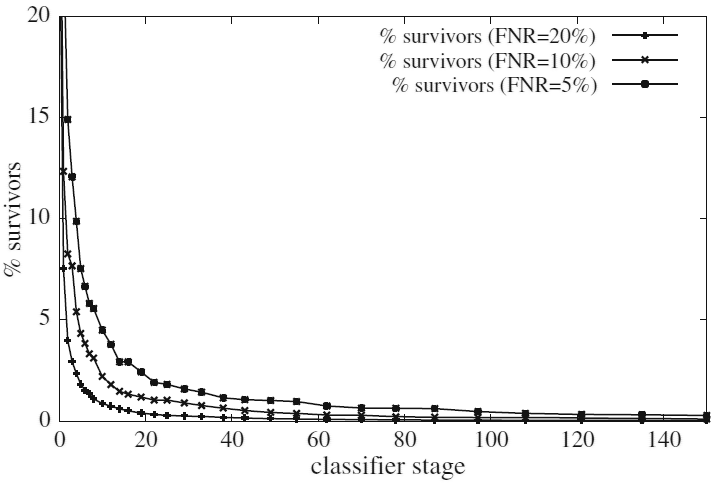
\includegraphics[width=0.6\linewidth]{fig/survivors.png}
	\caption{Surviving percentage of samples gets below 5\% after few initial stages. Taken from \cite{herout-realtime-cuda}.}
	\label{fig:survivors}
\end{figure}
\end{center}

\section{Research}

\subsection{Real-time object detection on CUDA by Herout et al., 2009}

Most of the current implementations of WaldBoost detectors are based on this work. As mentioned previously and shown in \ref{fig:survivors}, only a few samples are being processed after few initial stages. The rest of the samples still occupy GPU resources and wait for these to finish. To free these resources and use them accordingly, a method of thread rearrangement was proposed.

\subsubsection{Pyramidal image}

The detector uses a window for scanning the image, usually 24x24 or 26x26 pixels. In order to detect the object in such window, a pyramidal image was proposed. Such image contains many sub-sampled images stored in a pyramid fashion. The structure of the pyramidal image and the way how to construct it is discussed in \ref{subsubsec:pyramidal}.

\subsubsection{Thread rearrangement}

At the time of writing the paper, detectors with 512 or 1024 stages were used (this implementation uses a detector with 2048 stages). Herout et al. proposed, that every sample can be processed up to a set number of stages, after which thread rearrangement is done as described in \ref{fig:thread-rearrangement} and the process continues.

\begin{center}
\begin{figure}[h]
	\centering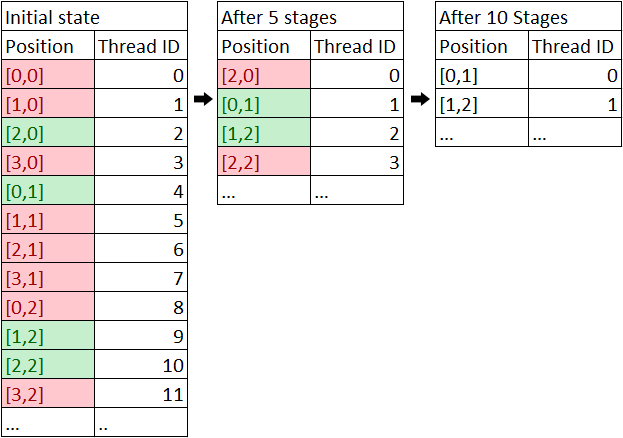
\includegraphics[width=0.6\linewidth]{fig/threadrear.png}
	\caption{Thread rearrangement of surviving threads (green) after 5 and 10 processed stages.}
	\label{fig:thread-rearrangement}
\end{figure}
\end{center}

Methods how to achieve this rearrangement are again specific to the implementation and are discussed later in \ref{subsec:thread-reorganization}.

\section{Tools to be used}

\subsection{Debugging and profiling}\label{subsec:debugging-and-profiling}

One of the main advantages of CUDA over OpenCL are its debugging and profiling environments, which are important for writing optimized and error-free code. There are several CUDA-specific options to use. CUDA Profiler API also provides functions to help with profiling. Only specific parts of the code can be profiled by using \verb|cudaProfilerStart| and \verb|cudaProfilerStop| calls. This allows to collect data only for important parts of the code.

\subsubsection{Visual Profiler}\label{subsubsec:visual-profiler}

The first option to profile and optimize code is the Visual Profiler. As the name itself says, it displays a visual representation of all the GPU calls, where statistics such as memory bandwidth (shared, local, global, \dots), instruction throughput, occupancy and much more can be displayed. It is well documented \footnote{\url{http://docs.nvidia.com/cuda/profiler-users-guide/\#visual-profiler}} and provides a simple interface to use (\ref{fig:visual-profiler}). 

\begin{figure}[h]
	\begin{center}
	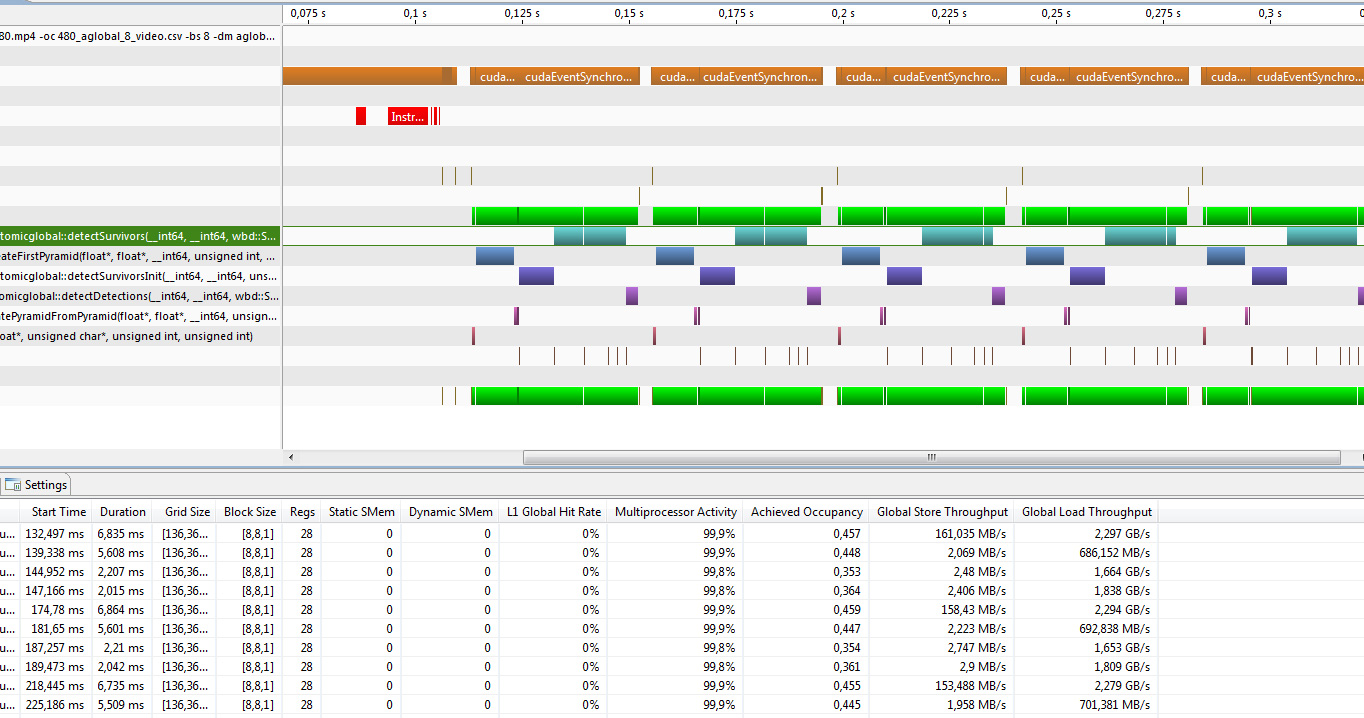
\includegraphics[width=0.8\textwidth]{fig/visual_profiler.jpg}
	\caption{Visual profiler interface.}
	\label{fig:visual-profiler}
	\end{center}
\end{figure}


To profile a program, only four things need to be set up: binary file to run, CUDA toolkit version, working directory and command line arguments. The profiler allows to export the results to a CSV file.

\subsubsection{nvprof}\label{subsubsec:nvprof}

Nvprof has basically the same options as the Visual Profiler, with the difference, that it is a command-line tool. As such it can be used as a part of a script, which can automate the whole process of profiling.

\begin{figure}
\begin{verbatim}
nvprof --analysis-metrics -o  myprog-analysis.nvprof ./myprog --benchmark -i=1
\end{verbatim}
\caption{An example how to run nvprof to output profiling data.}
\end{figure}

\subsubsection{NVIDIA Nsight}

Another handy tool to use is NVIDIA Nsight, which is a set of tools developed for Microsoft Visual Studio \footnote{\url{https://www.visualstudio.com/}} and Eclipse \footnote{\url{https://eclipse.org/}} allowing to debug and analyze GPU and graphics applications.

It consists of two main modules and allows for simple profiling. On the other hand dedicated tools such as \ref{subsubsec:visual-profiler} or \ref{subsubsec:nvprof} are better for the job.

\paragraph{CUDA Debugger} allows to set breakpoints inside GPU code and view the local variables, inspect the memory or perform other debugging tasks such as memory checks.

\paragraph{Graphics Debugger} allows to debug vertex shaders, pixel shaders and view the current state of the graphics pipeline.

\chapter{Implementation}\label{ch:implementation}

The object detector is implemented in C++ with dependencies on OpenCV\footnote{\url{http://www.opencv.org}} - an open source computer vision library with C and C++ interfaces and CUDA\footnote{\url{http://www.nvidia.com/object/cuda_home_new.html}} - a library for writing NVIDIA GPU code with a CUDA C interface, which is an extension to C compiled by the NVCC compiler.

It is implemented as an easy-to-use class, which takes a dataset or a video on the input and outputs detections. Current implementation uses an open-source face detector trained by R. Juranek\footnote{\url{http://medusa.fit.vutbr.cz/LBPDetector/}} under Brno University of Technology license. As such, it can be used as a part of an application such as face tracking or face recognition, but not only faces have to be processed. Depending on what detector is trained on, anything from traffic signs to humans can be detected.

\begin{center}
\begin{figure}[h]
	\centering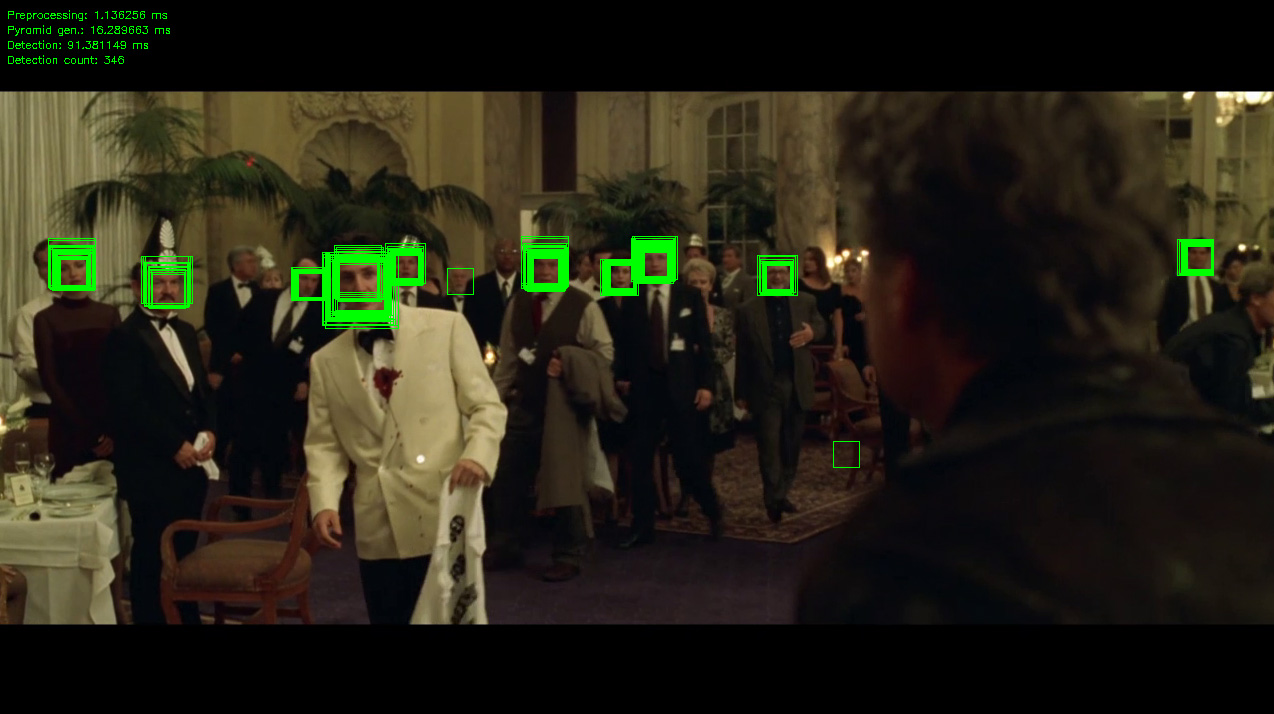
\includegraphics[width=0.8\textwidth]{fig/sample.jpg}
	\caption{A sample output with debug information shown.}
	\label{fig:sample}
\end{figure}
\end{center}

A CMake\footnote{\url{http://www.cmake.org/}} project is included, therefore it can be built on multiple platforms. As for the project itself, it is logically separated into the following modules and sub-modules (in code this is done using C++ namespaces):

\begin{itemize}
	\item wbd - wrapper around the whole detector
	\item wbd::simple - CPU implementation of the waldboost detector
	\item wbd::gpu - WaldboostDetector class, an interface to use the detector and most of the methods used for GPU acceleration
	\item wbd::gpu::pyramid - pyramidal image generation on the GPU
	\item wbd::gpu::detection - object detection on the GPU
\end{itemize}

\section{Detector}\label{sec:detector}

The detector can be used to detect any object it is trained to, not only faces. Most detectors are stored as XML files, which brings the overhead of reading and parsing a file and so an exported version of an XML detector to a C++ header file is used. As such 2 header files (\verb|wbd_detector.h|, \verb|wbd_alphas.h|) must be compiled with the detector.

These headers are be obtained by parsing a XML detector \footnote{\url{https://github.com/mmaci/classifier-export}}. The detector consists of two main parts, the stages (\ref{fig:stage}) or also called the weak classifiers, which are loaded into a structure \ref{fig:stage} and an $\alpha$-table, which is stored as an array of floating-point values. Every stage points to a specific range inside the $\alpha$-table, where responses for all the LBP values are stored. Training of a detector is not the subject of this thesis and as such it will not be discussed.

\begin{figure}[h!]
\begin{verbatim}
struct Stage {
    uint8 x, y; // X, Y offsets
    uint8 width, height; // width, height of the feature
    float thetaB; // threshold
    uint32 alphaOffset; // alpha table offset
};
\end{verbatim}
\caption{Stage structure}
\label{fig:stage}
\end{figure}

The detector uses a 26x26 pixel-wide scanning window, where \verb|x| and \verb|y| are offsets inside the window and \verb|width| and \verb|height| describe the size of the feature. It is the size of 1x1, 1x2, 2x1 or 2x2, because of this knowledge, hardware provided bilinear interpolation can be used. \verb|alphaOffset| is an offset inside the $\alpha$-table corresponding to appropriate LBP values. \verb|thetaB| is the threshold value, which decides if the sample gets discarded or not in the current stage.

\section{Interface}

The object detector is designed to be used using a class WaldboostDetector, to simplify the detection as much as possible it is able to be run only by loading a video or a dataset and then running the \verb|run()| method, which returns a list of detections. Optionally the programmer can set specific settings described such as the method used ir block configuration. On the other hand when not set, these are set optimally based on results obtained by measurements on different GPU's.

The whole interface is described in the added Doxygen\footnote{\url{http://www.doxygen.org}} documentation.

\section{Program cycle}

The detector processes both videos and image datasets, which are passed to the detector as a filename. For a dataset, a text file is used with filenames of the images separated by a newline. OpenCV is used to load both images and videos and as such it supports most common formats.

The application pipeline (\ref{fig:pipeline}) of the detector is a bit different for a dataset, than for a video, but both use the following steps as described in \ref{subsec:init} to \ref{subsec:free}.

\begin{center}
\begin{figure}[h!]
	\centering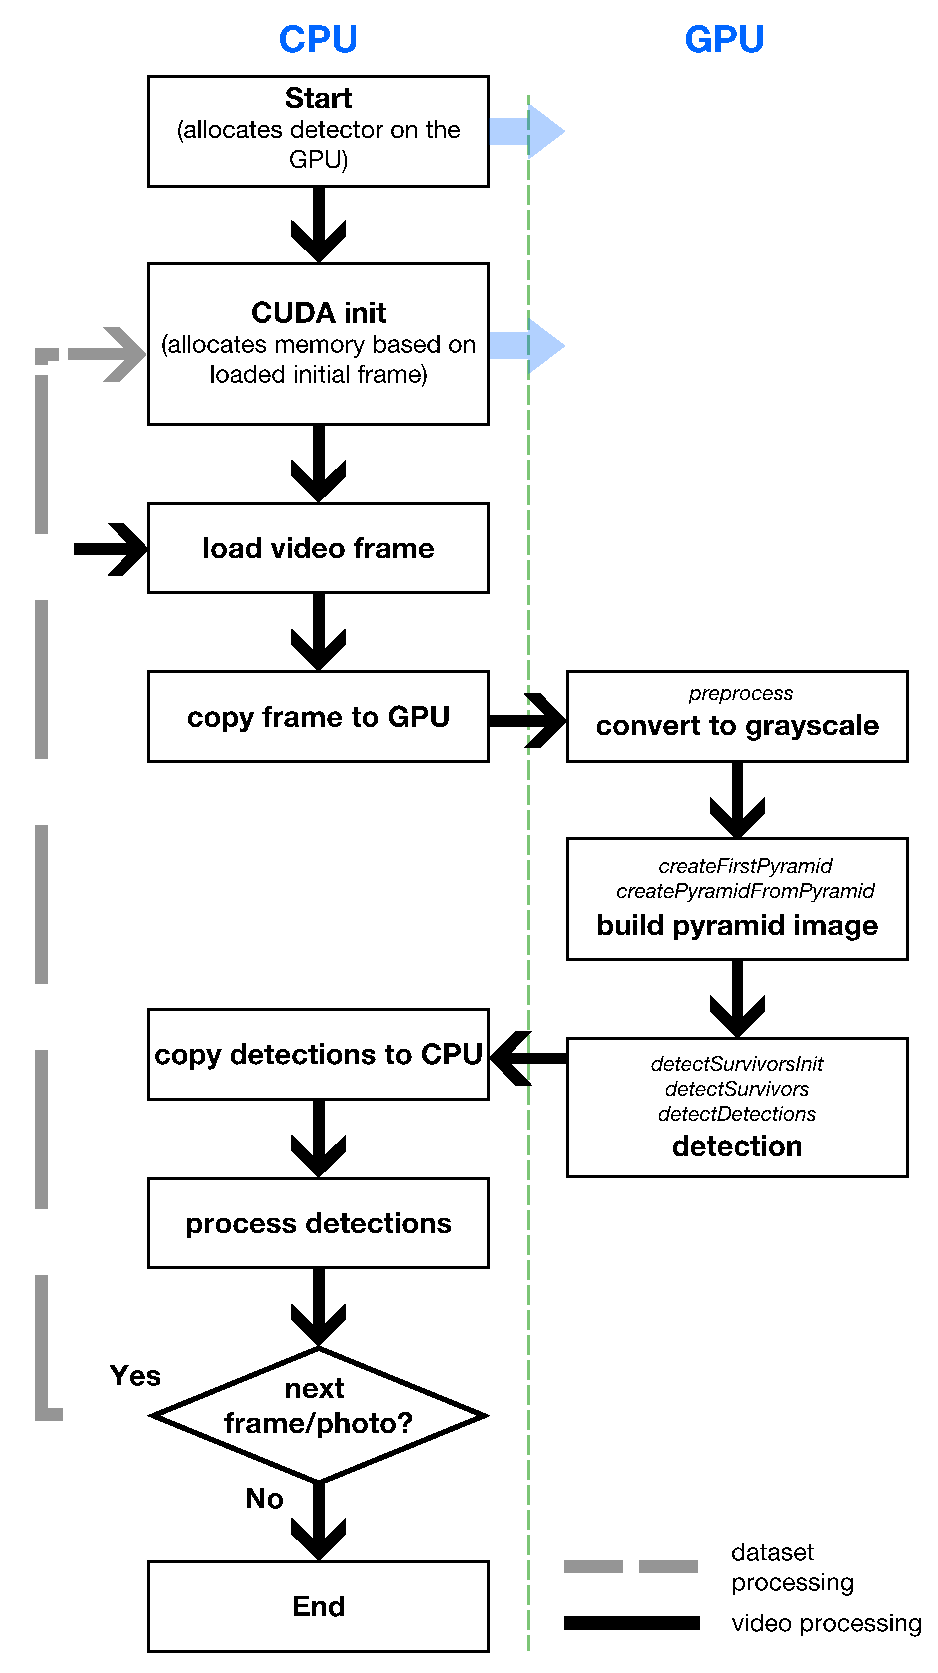
\includegraphics[width=9cm]{fig/pipeline.eps}
	\caption{Application pipeline. On the GPU side, kernel methods are mentioned.}
	\label{fig:pipeline}	
\end{figure}
\end{center}

For a video, the detector can be initialized only once with the initial frame. All the other frames have the same size and so the same memory structures can be used. Image setup and the Detection are then run multiple times for every frame. After the video is processed, memory is freed.

For a dataset, every image can be different and so the whole process must be run multiple times for every loaded image.

\subsection{Initialization}\label{subsec:init}

The initialization of the detector can be separated into two parts. The first being the tasks, that have to be done only once for both datasets and videos. This means copying the detector into GPU memory (the detector contains weak classifiers/stages and an $\alpha$-table). This is done in the constructor of the WaldboostDetector class.

The other part being allocating GPU memory for the image itself, which is allocated dynamically due to dependence on the size of the input image. For a video this can also be done only once, because every frame has the same size and as such, everything is allocated based on the initial frame. On the other hand a dataset can have completely different image sizes and so this must be done for every photo separately.

A method to skip multiple initialization for datasets was proposed and is discussed in \ref{subsec:dataset-texture}.

\subsection{Setting an image}

After the initialization is complete, an image or a frame is loaded by OpenCV and then copied over to the GPU. This must be done both for every image or every frame. It is copied over to the global memory, there it is preprocessed (\ref{subsubsec:grayscale}) and set as a texture. From the texture, a pyramidal image is generated (\ref{subsubsec:pyramidal}). After that, everything is ready for object detection.

\subsubsection{Preprocessing} \label{subsubsec:grayscale} 

The first kernel to be run is the preprocessing kernel. There are 2 operations to be done - conversion from the initial integers to a floating-point representation and then a conversion to grayscale.

Floats are needed in order to work with textures. Texture memory enables hardware implemented bilinear interpolation for subsampling images, which is done mainly in creating the pyramidal image (\ref{subsubsec:pyramidal}. Even though bilinear interpolation should only be supported for floating-point values, due to official documentation, it is not the case. On the other hand it might be a bug, which might get fixed in the future and it would be wise not to be used.

Conversion to grayscale is a simple image processing operation described by the formula \eqref{eq:rgbtograyscale}. The detector itself is trained on grayscale images, and so the input must also be in grayscale. After the kernel finishes, the result is saved as a texture.

\begin{equation} \label{eq:rgbtograyscale}
Y=0.2126R + 0.7152G + 0.0722B
\end{equation}

\subsubsection{Dynamic texture and texture objects}\label{subsubsec:dynamic-texture}

As of CUDA 5.0 and Kepler GPUs textures don't have to be defined globally as static textures, but they can be used dynamically using Texture Objects (\verb|cudaTextureObject_t| class API \cite{cuda-texture-obj}).

This has several advantages. One of them being the slight overhead (up to $1.5 \mu s$) by binding and unbinding static textures during kernel launch, which is eliminated. Even though this is not our case and doesn't sound as much, it might be quite a significant overhead while launching large quantities of fast kernels.

The main advantage in our case is, that texture objects can be passed as arguments, set to store variable image sizes and therefore easily be used as a part of a library. Also multiple textures can be created using given parameters, which is exploited in pyramidal image creation and explained in \ref{subsubsec:pyramidal}.

\subsubsection{Pyramidal image}\label{subsubsec:pyramidal}

All the pixels are processed using a 26x26 pixel-wide window. The size again depends on how the detector is trained. The basic idea is that for the given object, all the features describing it fit inside this window. On the other hand objects, such as faces, are usually much larger in the initial image, therefore we have to create many sub-sampled images and run the detection on every one of them. In order to do this a the second kernel to be run is the pyramid kernel.

The straight forward method is to create a single pyramidal image and store it as a texture on which the detection is run.

As mentioned previously, the implementation uses hardware bilinear interpolation provided by the texture memory for sub-sampling the image. It has to be kept in mind, that bilinear interpolation has some negative side-effects, one of them being the sub-sampling of an image below half its original width.

\begin{center}
\begin{figure}[h]
	\centering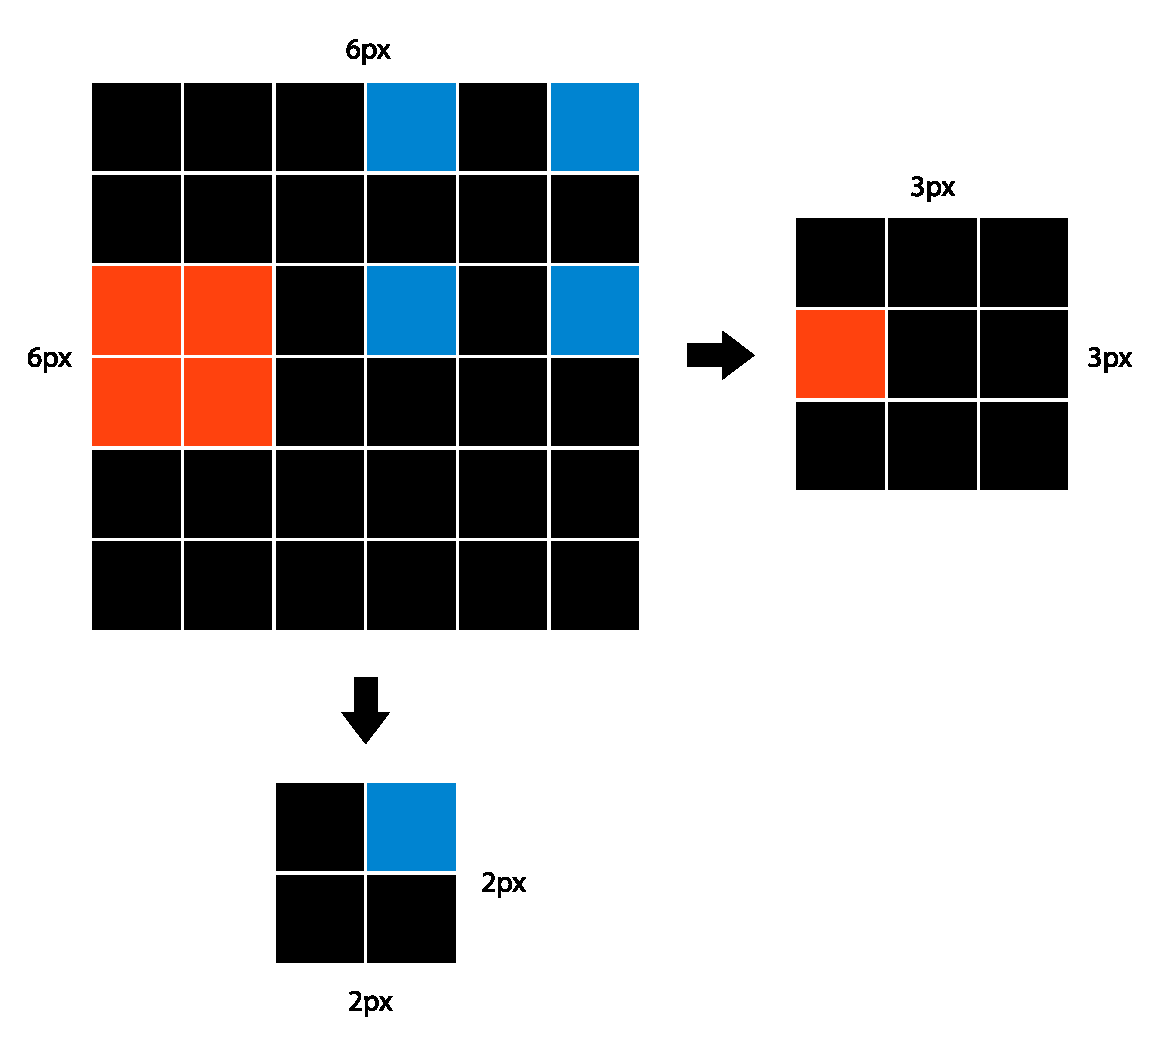
\includegraphics[height=9cm]{fig/bilinear_error.eps}\label{fig:bilinear-error}
	\caption{Error when sub-sampling an image below twice the original width using bilinear interpolation}
\end{figure}
\end{center}

As shown on \ref{fig:bilinear-error} when sub-sampling an image below half its original width, pixels are left out and a sampling error is created. Other methods, such as Lanczos resampling, solve this at the cost of a computational overhead, because a software implementation has to be used instead of the hardware-based provided by using a floating-point 2D texture.

The image is generated in octaves. An octave is a structure of several images, where the smallest image has half the width/height of the original image. Depending on the number of images in an octave, every image is $2^1/number_of_images$ smaller than the previous. The following octave is then sub-sampled from the previous octave.

Two methods were tested. The first one using a single texture for both writing a reading the individual octaves. This proved to be very costly and therefore another method had been implemented and is described below:

\begin{enumerate}
	\item A pyramidal image of $N$ images is generated, where each image is $2^1/N$ smaller then the previous. Every image is sub-sampled from the original image.
	\item Generated pyramidal image is stored as a dynamic texture. Simultaneously the pyramid is being written inside a final image used for detection.
	\item A pyramidal image is generated, by sub-sampling the previously generated pyramid. Width and height of the sub-sampled pyramid are twice smaller than that of the original.
	\item Generated pyramidal image is saved as a dynamic texture.
	\item Steps 3 and 4 get repeated for a set number of octaves.
\end{enumerate}

\begin{center}
\begin{figure}[h]
	\centering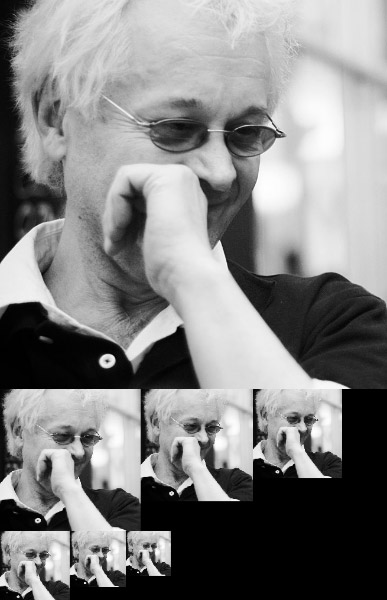
\includegraphics[height=9cm]{fig/pyramid.jpg}
	\caption{Pyramidal image}
\end{figure}
\end{center}

The implementation itself uses 8 levels and 4 octaves. This results in the sides of the smallest image being 16x smaller than the original. By reducing the number of octaves or levels, better performance can be gained at a cost of the quality of the detections.

\subsection{Detection}

To detect an object, the detector has to successfully evaluate a given number of stages (weak classifiers) described in \ref{sec:detector}, which are processed sequentially. In our case 2048. This number can be reduced, but it will have an impact on the number of detections. Every weak classifier the algorithm processes, a response is given. The response is a number read from the $\alpha$-table, from the address given by the stage offset and the calculated LBP value. It is then added to the accumulated response. The sample is discarded in case the accumulated value falls below the stage threshold \verb|thetaB|.

\begin{algorithm} \label{alg:detection}
\For{every pixel (a GPU thread is created)}
{
	\For{every stage}
	{
		1. compute LBP coefficient \\
		2. add response for the given LBP to the accumulated response \\
		\If{accumulated response $\geq$ stage threshold $thetaB$}{
			discard sample
		}
	}
}

\caption{Object detection algorithm simplified}
\end{algorithm}

\subsection{Freeing the memory}\label{subsec:free}

After everything has been processed, the GPU memory can be freed. This also must be done for every image in case of a dataset, but only once in case of a video.

\section{Memory organization} \label{sec:memory-organization}

The use of GPU memory is one of the most important parts of programming on GPU architectures. The types of CUDA memories are described in \ref{subsec:memory}.

Below we will discuss, how the most important parts of the detector are stored and why.

\begin{itemize}
\item \textbf{Stages/Weak classifiers} - constant memory \\
Stages are stored in the constant memory. Even though it's not as fast as let's say shared memory, its capability to broadcast simultaneously accessed data is ideal. Every thread processes a single image position, for which it loops through a for-cycle of stages. Every read from the constant memory is then not only broadcast to a half-warp (a group of 16 threads), but also cached. The only problem can be the size, which is limited to 64 KB. The detector uses 2048 stages, where each stage is 12 B. This leads to 24 KB, which is enough, but has to be accounted for when storing other data in the constant memory.

\item \textbf{$\alpha$-table} - texture memory \\
There are 256 coefficients for every stage and every coefficient is stored as a float. This leads to $256 * 2048 * 4 = 2 MB$ and by far exceeds the memory available for constant memory. Another reason the constant memory cannot be used is that the access is random, due to the fact, that we are likely to get different LBP values for every pixel. In this case we wouldn't utilize the broadcast and it would even be slower.

\item \textbf{Original image and pyramidal image} - texture memory \\
Both are stored in the texture memory. Original image is used to create a pyramidal image using hardware accelerated bilinear interpolation for creating down-sampled images as described in \ref{subsubsec:pyramidal}. It is highly optimized for random read-only access, which is exactly what we want.
\end{itemize}

\section{Thread allocation}\label{sec:thread-alloc}

A GPU thread is allocated for every sample, therefore every pixel/sample. Based on \cite{herout-realtime-cuda} only a fraction of samples (around 1\%) is still processed by the classifier after the few initial stages. On the other hand the GPU organizes threads in warps - groups of 32 threads, which are organized in blocks across with they can be synchronized. The problem is, that when only a single thread within a warp is active, the other threads have to wait for it until it finishes, thus wasting GPU resources.

\section{Thread reorganization}\label{subsec:thread-reorganization}

\cite{herout-realtime-cuda} proposed, that every few stages threads can be checked if they are still evaluating the classifier stages or they have been dropped. Surviving threads can then be reorganized and continue with evaluating the weak classifiers.

The detector uses several ways of reorganizing surviving threads. Every one of them works better under different conditions. They are summarized below by the types of functions and memory used.

\begin{itemize}
	\item atomic functions / global memory
	\item atomic functions / shared memory
	\item atomic functions / hybrid global-shared
	\item prefix sum / global memory
\end{itemize}

The whole implementation is based around three functions, which are implemented as \verb|__device__| functions in case of the shared memory implementation, otherwise they are kernels on their own. The shared memory is specific by the fact, that it operates only within shared memory space and doesn't use global memory at all and as such, it doesn't have to be synchronized by rerunning the whole kernel.

\begin{itemize}
	\item \verb|detectSurvivorsInit| - processes all samples for a given number of stages and outputs the surviving threads. Called at the beginning.
	\item \verb|detectSurvivors| - processes surviving samples for a given number of stages and outputs the surviving threads. Called multiple times.
	\item \verb|detectDetections| - processes remaining surviving threads and outputs detections. Called at the end.
\end{itemize}

\subsection{Atomic functions and global memory} \label{subsec:afgm}

The first proposed method uses a counter stored in global memory to count the number of surviving threads within a block and global memory for storing the surviving sample information. After processing a given number of stages of a classifier, every sample which wasn't discarded by the classifier is assigned an ID in global memory by reading the current value of the surviving sample counter and incrementing it. It then saves the information about the surviving sample (\ref{fig:survivordata}) to global memory based on the assigned ID.

\begin{figure}[h!] \label{fig:survivordata}
\begin{verbatim}
struct SurvivorData {
    uint32 x, y; // X, Y coordinates of the sample
    float response; // current response
};
\end{verbatim}
\caption{Stage structure}
\end{figure}

Threads cannot be synchronized across the whole grid, which means, that it is not possible for all the samples to stop at a given stage and write down the surviving samples. In other words, it is possible, that a thread processing survivors after, let's say 512 samples, would write to memory at the same time, as another thread processing survivors after 256 stages, therefore a new kernel must be launched.

\subsubsection{Advantages}

\begin{itemize}
	\item Samples are tightly packed together after synchronization, using up as little memory (and warps) as possible.
\end{itemize}

\subsubsection{Disadvantages}

\begin{itemize}
	\item A global memory counter might become a serious bottleneck on an image with a lot of detections, because threads will get stalled waiting for the atomic increment to be processed.
	\item The use of global memory is generally slow, even though it can be optimized by coalescing (\ref{subsubsec:coalescing}).
	\item An overhead of running a new kernel.
\end{itemize}

\subsection{Atomic functions and shared memory}\label{subsec:afsm}

To solve these issues a method exploiting the use of shared memory was proposed. All the survivors are stored in shared memory and so is the counter, which only counts surviving threads within a block. This means, that all the threads are processed locally within their block.

Functions are not implemented as kernels, like in the previous case, but only as \verb|__device__| functions. The kernel doesn't have to be run again,  in this case.

After processing a given number of stages the surviving sample is assigned an ID based on the value of the counter, which is a number ranging from 0 to max threads per block and atomically increments it. Threads are then synchronized and evaluation of the stages continues. This leads to warps being freed.

\subsubsection{Advantages}

\begin{itemize}
	\item Shared memory is much faster than global memory (the bandwidth of shared memory is ~1.7TB/s compared to that of global memory which is ~150GB/s.
	\item Counters and atomic increments are distributed across shared memory removing the single counter bottleneck, as threads increment their counter separately based on the block they are in.
	\item Only a single kernel can be run with the use of \verb|__syncthreads| to synchronize threads inside a block every given stage.
\end{itemize}

\subsubsection{Disadvantages}

\begin{itemize}
	\item More warps are being run, because as long as there is at least a single sample being processed a warp has to be scheduled and the same happens for the whole block. As long as there is a single warp surviving inside a block, the block occupies a multiprocessor.
	\item An overhead of synchronizing threads, resetting the counter and checking for surviving threads is added.
\end{itemize}

\subsection{Hybrid method using both shared and global memory}\label{subsec:hybrid}

The overhead of rerunning a kernel is quite low and so a third method was proposed, which would solve the issue with having a lot of resources wasted on only a few threads occupying whole warps or blocks.

The hybrid method removes the global memory counter bottleneck and still preserves the efficiency of organizing survivors in global memory. It uses two counters, a local counter stored in shared memory, which assigns a local ID the same way as in \ref{subsec:afsm} and a global counter, which gets increased by the total number of its survivors. Adding to the global counter can happen only when a block is synchronized, because a final number of survivors within a block must be known. It is used as an offset to the global memory array for the block of surviving samples, whereas the local counter is used an offset within this block of memory.

Basically this method can be looked at as a compromise between the global memory implementation (\ref{subsec:afgm}) and the shared memory implementation (\ref{subsec:afsm}).

\subsubsection{Advantages}

\begin{itemize}
	\item Distributed use of counters. The maximum number of atomic increments inside a block is the size of the block and the maximum number of atomic adds to the global counter is the number of blocks.
	\item An efficient use of global memory and GPU resources by tightly storing the surviving samples.
\end{itemize}

\subsubsection{Disadvantages}

\begin{itemize}
	\item Synchronization of a block is needed before the global counter can be added to, which stalls a large portion of the threads inside a block.
	\item An overhead of running new kernels.
\end{itemize}

\subsection{Prefix-sum}\label{sec:prefixsum}

The last proposed method tries to remove the use of a counter altogether and thus removing a possible bottleneck. A parallel prefix-sum is an algorithm commonly used for such tasks. It allows to sum up values on a parallel architecture with a logarithmic complexity.

The main idea behind is, that it produces an array of values, where every element is the sum of the previous values. For an array of 0's and 1's, where 1 is a surviving thread and 0 is a discarded thread, it not sums up all the survivors in the last element, but also assigns a unique id for every thread. This is done using shared memory, where the size of the memory is the same as the number of threads in a block.

The algorithm can be viewed as a tree and be represented as an array in shared memory. It consists of two phases an up-sweep phase and a down-sweep phase. The tree is a binary tree with the values (in our case 1's and 0's) as leaves.

In the up-sweep phase, the tree is traversed from its leaves to the root, where in every stage the values are summed up in their parent as shown in \ref{fig:sweepup}.

\begin{center}
\begin{figure}[h]
	\centering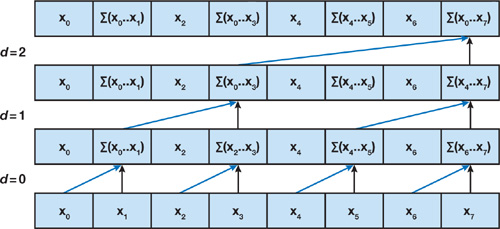
\includegraphics[width=0.6\linewidth]{fig/sweepup.jpg}
	\caption{Up-sweep phase of the prefix sum algorithm (taken from \cite{gems-prefixsum})}
	\label{fig:sweepup}
\end{figure}
\end{center}

At the beginning half of the threads in a block are used to calculate the corresponding sums. The next iteration the number of threads used is halved and so on, until the root is reached, in which the total sum of all the values is stored.

In the down-sweep phase as shown in \ref{fig:sweepdown}, the root is zeroed and traversed back to the leaves. Using the partial sums a sum of all the previous values for every leaf is gained.

Every surviving thread is then assigned an ID based on its value in the prefix-sum array and the total number of surviving threads inside the block is the last value inside the array.

\begin{center}
\begin{figure}[h]
	\centering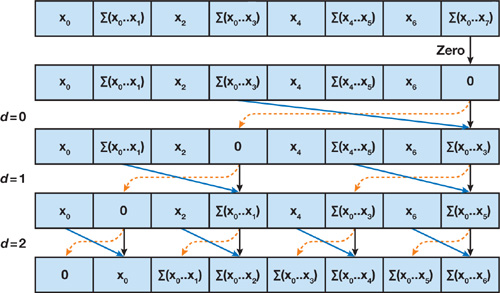
\includegraphics[width=0.6\linewidth]{fig/sweepdown.jpg}
	\caption{Down-sweep phase of the prefix sum algorithm (taken from \cite{gems-prefixsum})}
	\label{fig:sweepdown}
\end{figure}
\end{center}

\section{Setting the thread-reorganization stages}

Thread reorganization is a costly process, but greatly enhances the performance, therefore a balance between reorganizing threads and running the detection has to be found. As described thoroughly in \ref{subsec:thread-reorganization}, every detection function call has a starting stage and an ending stage. For the initial function call, the stating stage is set to 0 and for the final stage as the number of stages - in our case 2048. It is then quite important to set these, because it will have large impact on the overall performance.

The proposed strategy is to reorganize threads every time the number of surviving threads is half the original value of surviving threads. It is quite unthinkable to do this performance-wise. The kernel would have to be run for every stage and the number of surviving threads copied to the host memory. 

Scenarios for low-detection count (one or two faces, 10's of detections) and high-detection count (a group of faces, 100's of detections) were run stage by stage, measuring the average stage, in which the number of survivors is half the original. From this strategies were defined, which can be passed to the detector as an argument. These strategies are optimized for the current face detector, but as they are passed as a vector of values, it is easy to extend the detector with other strategies.

\chapter{Performance measurements and profiling}

This chapter evaluates performance results obtained by measurements on different GPUs and discusses them based on results obtained from profiling.

The technology used in the implementation  is supported only by the Kepler architecture and newer (CUDA 5.0+). Because of this the cutting edge Kepler and Maxwell GPU's were chosen (GTX 980 for the Maxwell architecture and GTX 780Ti for the Kepler architecture) to test the limits of the implementation. Also an average notebook GPU (Quadro K1000M) was used to test the performance in more standard user conditions. Specifications of the GPU's can be found in \ref{tab:parameters-gpu}. The driver version used was 340.62 and for the CPU Intel(R) Core(TM) i7-3610QM CPU @ 2.30 GHz. The discussion focuses on the best results obtained by every GPU.

The tested use cases were the following:

\begin{itemize}
	\item 720x480 video
	\item 1280x720 video
	\item 1920x1080 video
	\item BioID face dataset with 1512 grayscale images
\end{itemize}

As a video a section of the movie "The Game" (1997) with a larger group of people, having ~10-50 faces per frame.

\begin{center}
\begin{table}[htbp]
\begin{tabularx}{\textwidth}{| X | X | X | X |}
\hline
- & NVidia GeForce GTX 980 & NVidia GeForce GTX 780Ti & NVidia Quadro K1000M \\
\hline
Architecture & Maxwell & Kepler & Kepler \\
\hline
SM's\footnote{Streaming multiprocessors} & 16 & 15 & 1 \\
\hline
CUDA Cores\footnote{Depends on the architecture. Maxwell has 128 CUDA cores per SM, whereas Kepler has 192 CUDA cores.} & 2048 & 2880 & 192 \\
\hline
Base Clock (MHz) & 1126 & 875 & 850 \\
\hline
Memory (MB) & 4096 & 3072 & 2048 \\
\hline
Memory bandwidth (GB/s) & 224 & 336 & 28.8 \\
\hline
\end{tabularx}
\caption{Parameters of graphics cards used for performance measurements}
\label{tab:parameters-gpu}
\end{table}
\end{center}

Another important thing to mention is the Compute Capabilities the object detector is targeted are 3.0 for the Kepler architecture cards and 5.0 for the Maxwell architecture GeForce GTX 980. The limits of the architectures are summarized in \ref{tab:capability-3050}. Most of the measurements discussed in \ref{sec:detection-time} will depend on these limits and so it is important to take them into consideration.

\section{Detection time}\label{sec:detection-time}

In order for the detector to be a real-time object detector, it must process the video in under $1/framerate$ seconds. Therefore, the main focus of the measurements was on the detection time of the individual kernels.

As mentioned in \ref{subsubsec:thread-hierarchy} the kernels are initialized with a thread configuration, which can be 1D, 2D or 3D. In our case the following 2D configurations were used: 8x8 (64 threads per block), 16x16 (256 threads per block), 32x32 (1024 threads per block). The most important things, that depend on the size of a block are the size of the shared memory and the number of threads, which are synchronized using the \verb|__syncthreads| call. Only $2^N$ sizes of the blocks were tested, because specifically the prefix-sum implementation works only for those.

\subsection{Global and shared memory usage}

\begin{figure}
	\label{fig:quadro-det-measurement}
	\centering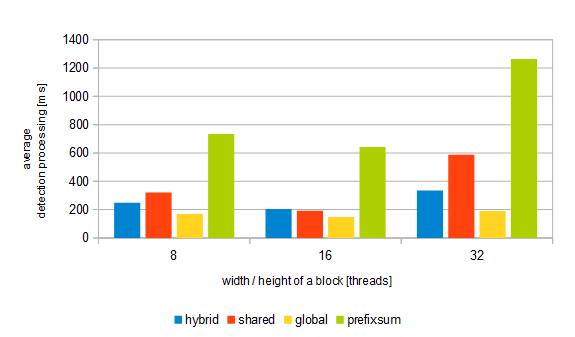
\includegraphics[width=0.85\textwidth]{fig/1080_detection_quadrok1000m.png}
	\caption{Comparison of detection times of different implementations on Quadro K1000M (Kepler)}
\end{figure}

The most interesting thing to note is that, for the Quadro K1000M, the fastest implementation is actually the global memory implementation. Originally it was thought, that the fastest implementations would be the shared (\ref{subsec:afsm}) or the hybrid-shared methods (\ref{subsec:hybrid}), because of the idea of having a single counter in global memory and all the threads getting stalled. 

The real bottleneck seems to be the single multiprocessor, which in the case of of the shared memory implementation, doesn't process the blocks fast enough. This can be seen in \ref{fig:quadro-det-measurement}, for the 8x8 kernel, where the shared memory implementation is slower, than the hybrid-shared due to the fact, that the configuration consists of a lot of blocks, which are used only by a few threads.

\subsection{Selecting the optimal block configuration}\label{subsec:block-config}

In all of the measurements (\ref{fig:quadro-det-measurement}, \ref{fig:780ti-det-measurement} and \ref{fig:980-det-measurement}) the best results were obtained for the 16x16 configuration, with the exception of the global memory implementation, which wasn't affected all that much by the configuration. For the Maxwell architecture, the best results were actually obtained by the 32x32 configuration.

The main reason, the global memory implementation wasn't affected that much is, that the main bottleneck is the global memory counter. It doesn't depend much on how the threads are divided into blocks, as long as the multiprocessor is occupied, the stalls by the atomic increments are on per-thread basis and don't depend on the configuration.

\subsection{Shared memory and block size}

The size of the block affects the shared memory implementation the most, because the samples within a block share a counter, therefore the larger the number of threads withing a block, the more stalls by the atomic increments of the counter. This would lead to the conclusion, that the smaller the block the better.


\begin{figure}
	\label{fig:980-det-measurement}
	\centering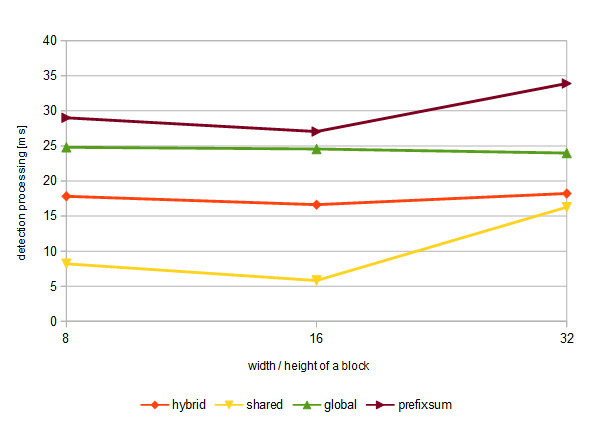
\includegraphics[width=0.85\textwidth]{fig/1080_detection_maxwell.png}
	\caption{Comparison of detection times of different implementations on GeForce GTX 980 (Maxwell)}
\end{figure}

\begin{figure}
	\label{fig:780ti-det-measurement}
	\centering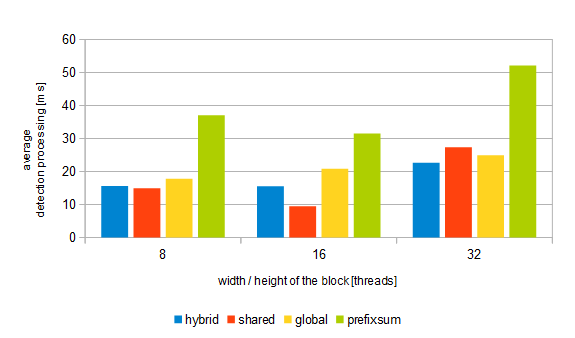
\includegraphics[width=0.85\textwidth]{fig/1080_detection_kepler.png}
	\caption{Comparison of detection times of different implementations on GeForce GTX 780Ti (Kepler)}
\end{figure}

It is however not the case, because of thread occupancy. The Kepler and Maxwell architectures have their limits of blocks per multiprocessor or warps per block, as mentioned in \ref{tab:capability-3050}. As such, even though the 8x8 configuration performs better, than the 32x32, and in terms of stalls even better, than the 16x16, it is not occupied to its maximum. Occupancy is discussed later on in \ref{subsec:occupancy}.

\subsection{Hybrid-shared memory method}

The hybrid-shared memory method, which was originally thought to be the most effective, didn't perform that well at the end. For the high-end GPU's, it performed worse in most cases, than the shared memory implementation. A huge difference between the two can be seen for the Maxwell architecture in \ref{fig:980-det-measurement}. This seems to be because of the great improvement of shared memory atomic operations in Maxwell.

\begin{figure}
\textit{"Maxwell improves upon this by implementing native shared memory atomic operations for 32-bit integers and native shared memory 32-bit and 64-bit compare-and-swap (CAS), which can be used to implement other atomic functions with reduced overhead compared to the Fermi and Kepler methods."}
\caption{Quoted from 1.4.3.3 Fast Shared Memory Atomics in \cite{cuda-toolkit-docs}}
\end{figure}

For the Kepler architecture GPU's it performed slightly worse for the GTX 780Ti and better for the Quadro K1000M, than the shared memory method. This is a result of the GTX 780Ti having 16 streaming multiprocessors, which get occupied by the larger number of blocks with the shared memory method, whereas for the Quadro K1000M, its single multiprocessor becomes the bottleneck.

\subsection{Prefix-sum}

The prefix-sum implementation performed worse in terms of detection time, than all the other implementations using atomic methods. This is due to the algorithm design, where all the threads inside a block have to be synchronized and wait for a single thread to read the thread offset. All the warps inside a block are therefore stalled until the very end, where the number of surviving threads is finally calculated.

\subsection{Summary}

In terms of the best implementation for a given GPU, the implementation was tested on high-end Kepler and Maxwell GPU's with 16 and 15 multiprocessors and an average Kepler GPU with a single multiprocessor. The proposed methods to use with these are the following:

\begin{table}[htbp]
\label{tab:proposed-methods}
\centering
\begin{tabular}{| l | l | l | l | l |}
\hline
Category & Proposed method \\
\hline
high-end Maxwell & 16x16 shared memory implementation \\
\hline
high-end Kepler & 16x16 shared memory implementation \\
\hline
Average Kepler & 16x16 global memory implementation \\
\hline
\end{tabular}
\caption{Proposed implementation to be used for each configuration.}
\end{table}

\section{Profiling details}

Even though performance-wise all the implementations were already evaluated, in the following sections, details effecting the performance will be discussed. Compared to other GPU technologies, CUDA allows for profiling tools mentions in \ref{subsec:debugging-and-profiling}.

Implementations, which were proposed to be working the best performance-wise, were profiled for every GPU to confirm the assumptions made based on the detection time results.

\subsection{Achieved occupancy}\label{subsec:occupancy}

Achieved occupancy is the number of active warps per clock cycle divided by the maximum warps per multiprocessor and is one of the key factors influencing the detection time. It is important to note, that maximum occupancy doesn't always lead to the best results, because other areas of optimization, such as memory access or atomic operation stalls may outperform it. That is why memory throughput, both shared and global, depending on the implementation type, will also be discussed.

\subsection{Memory load/store throughput}\label{subsec:memory-throughtput}

Memory throughput is the data transferred by the kernel per second, either by writing into the memory (store) or reading from it (load). For the global memory implementation, global memory throughput is measured, whereas for the shared memory implementation, its the shared memory throughput.

\subsection{Atomics throughput}\label{subsec:atomics-throughput}

Currently (Visual Profiler 6.5) it is hard to measure how the execution gets stalled by atomic operations, therefore atomic throughput is measured, which correlates with this. The higher the throughput, the less stalls are performed.

\subsection{Quadro K1000M (Kepler)}

\subsubsection{Achieved occupancy}\label{subsubsec:ach-occupancy}

\begin{figure}[h]
	\centering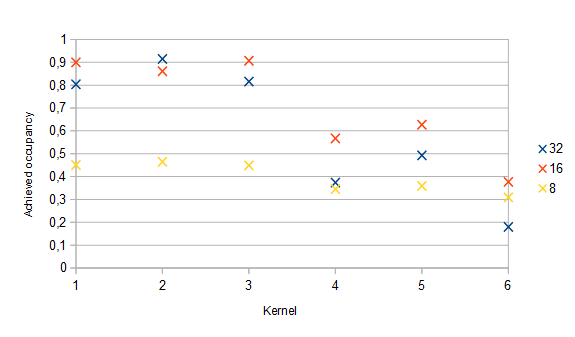
\includegraphics[width=0.85\textwidth]{fig/achievedoc_quadro.png}
	\caption{Achieved occupancy on Quadro K1000M (Kepler) for the global memory method. The numbers 1-6 enumerate the kernels, where 1 is the detectSurvivorsInit kernel, 2-5 are detectSurvivors kernels and 6 is the final detectDetections kernel.}
	\label{fig:occupancy-quadro}
\end{figure}

There are several things to note here. The first is the low occupancy of the 8x8 configuration, which varies between 30.9\% and 46.5\%. This can actually be predicted from \ref{tab:capability-3050}, where maximum number of blocks per streaming multiprocessor for compute capability 3.0 is 16, but the maximum number of threads is 2048. This means, that to reach full or almost full occupancy, at least 128 threads per block are needed. In case of 8x8 configuration, there are only 64 threads and so the maximum of 50\% occupancy for such configuration can be reached.

On the other hand for the last 3 kernels the occupancy is lower for all 3 configurations anyway, because the number of surviving samples is lower than the maximum occupancy. Lower occupancy doesn't always mean worse performance. In the case of the global memory implementation, even though the achieved occupancy of the 8x8 configuration is around 50\% of the 16x16 configuration, other factors such as atomic instruction usage actually perform better, even though they don't outperform it due to the low achieved occupancy.

\subsubsection{Global memory and atomic throughput}

Global memory load (\ref{fig:load-g-throughput}), store (\ref{fig:store-g-throughput}) and the atomic throughput (\ref{fig:atomics-throughput}) correlate with each other. The main bottleneck here is actually the use of atomic operations before the global memory stores are processed and so the store throughput is only as high as the atomic throughput.

\begin{figure}[h]
	\label{fig:load-g-throughput}
	\centering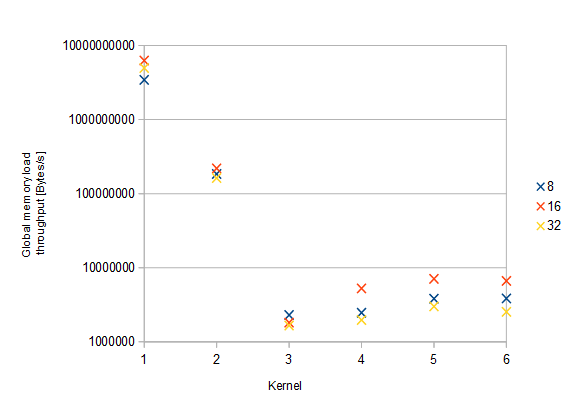
\includegraphics[width=0.85\textwidth]{fig/load_gthroughput_quadro.png}
	\caption{Load global memory throughput on Quadro K1000M (Kepler) for the global memory method. The numbers 1-5 enumerate the kernels, where 1-4 are detectSurvivors kernels and 6 is the final detectDetections kernel.}
\end{figure}

\begin{figure}[h]
	\label{fig:store-g-throughput}
	\centering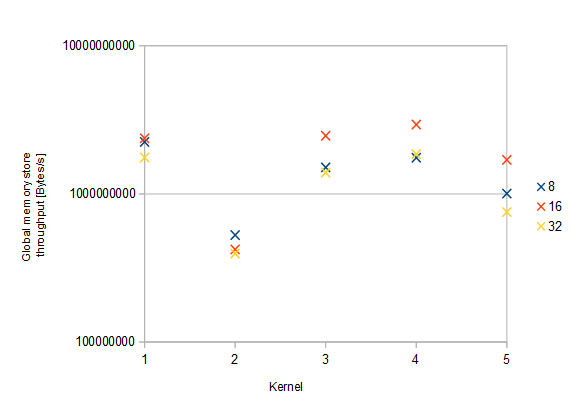
\includegraphics[width=0.85\textwidth]{fig/store_gthroughput_quadro.png}
	\caption{Store global memory throughput on Quadro K1000M (Kepler) for the global memory method. The numbers 1-6 enumerate the kernels, where 1 is the detectSurvivorsInit kernel, 2-5 are detectSurvivors kernels.}
\end{figure}

\begin{figure}[h]
	\label{fig:atomics-throughput}
	\centering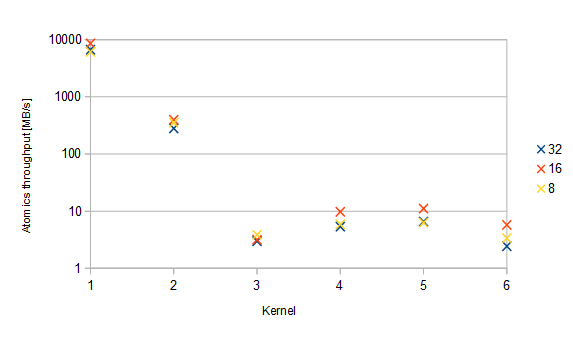
\includegraphics[width=0.85\textwidth]{fig/atomics_throughput_quadro.png}
	\caption{Atomic throughput on Quadro K1000M (Kepler) for the global memory method. The numbers 1-6 enumerate the kernels, where 1 is the detectSurvivorsInit kernel, 2-5 are detectSurvivors kernels and 6 is the final detectDetections kernel.}
\end{figure}

Again there are two things to be considered here discussed in \ref{subsubsec:ach-occupancy}. The 8x8 has a lower occupancy and the 32x32 creates more conflicts when issuing atomic operations, this leads to 16x16 being the best compromise between the two.

\clearpage

\subsection{GTX 780Ti (Kepler)}

% todo
TODO (will be measured on 18/05/2014).

\subsection{GTX 980 (Maxwell)}

% todo
TODO (will be measured on 18/05/2014).

\chapter{Summary}

The goal of this thesis was to design an application or a library for object detection on the GPU. The topic of WaldBoost object detection on the GPU using LBP is well researched, on the other hand there is much less research done on the implementation itself, and so the main focus was to exploit the implementation options of the NVidia CUDA Toolkit.

Different approaches to implement the detector were proposed, concentrating on the use of specific features of the GPU programming, to exploit the different bottlenecks of each method, and each on of them was thoroughly measured and profiled. The implementation itself then exploits the fact, that every GPU is very specific and can take advantage of a different feature of the NVidia CUDA Toolkit. As such, based on the GPU parameters, an optimal method for object detection can be run.

The detector\footnote{Latest version is available at: \url{https://github.com/mmaci/vutbr-fit-object-detection}} can process both image datasets, independent on the image size and videos, outputting detections as regions of interest inside an image. It can also be used as a part of another application, which uses object detection and it already was, as mentioned in \ref{subsec:face-tracking}. The application is specifically optimized not only for top-end NVidia GPU's, but also for the average or the low-end ones.

\section{Proposed improvements}

Throughout the thesis different methods how to optimize the detector were researched. Some of them were not yet implemented and measured. The ideas on which to focus in the future are the following:

\begin{itemize}
	\item \textbf{Measurements and profiling on more GPU's}. It was clear, that for the high-end GPU's the best results were obtained by the shared memory implementation and for the opposite extreme - a single multiprocessor GPU, the best results were measured for the global memory implementation. The hybrid-shared memory method didn't perform badly, but there were better tools for the job. GPU's such as the GTX 960, which has 8 streaming multiprocessors weren't available and it might be the case, that a middle way between the two optimal implementations might work the best.
	\item \textbf{Processing more stages.} Even on a GPU with a single streaming multiprocessor, the occupancy fell below 50\% for most of the stages and GPU resources were left unused. These resources might be used to process future stages and use them in a similar fashion as a cache. A way of mapping such stages, which were preprocessed to the ones being processed has to be proposed.
	\item \textbf{Prefix-sum.} The prefix-sum method should be researched more, if it can be optimized to discard unused threads throughout the computation.
	\item \textbf{Dataset initialization overhead.} When processing a dataset, GPU memory is allocated and freed specifically for every image. This brings a lot of overhead to the whole process, an overhead almost as large as the detection itself. A single texture can be allocated to copy the images to. The size of such has to be discussed, as it will stay the same throughout processing the whole dataset.
	\item \textbf{Minimize size of the block for shared memory implementation.} We found out, that even though 16x16 configuration performed the best, 8x8 configuration had good results, even though it had very low occupancy. Based on the architecture, a strategy can be devised for the size of the block, to be as small as possible and still fully occupy the GPU.
\end{itemize}


%=========================================================================

\nocite{zemcik-high-performance}
\nocite{herout-realtime-cuda}
\nocite{warps-occupancy}
\nocite{memory-coalescing}
\nocite{gpu-opt-fundamentals}